\chapter{The Neuro-Symbolic Paradigm: Bridging Statistical GNNs and Symbolic Oracles}
\label{ch:neuro_symbolic}

\section{The Core Dilemma: Shortcut Learning in Security GNNs}
The empirical results established in Chapter~\ref{ch:evaluation} present a profound scientific paradox:
\begin{itemize}
    \item On in-distribution enterprise data, CertGraph achieves near-perfect classification (Macro-F1 = $0.9986$), outperforming signature-based heuristics by $+28\%$.
    \item Under zero-shot adversarial hard negatives, CertGraph's accuracy collapses catastrophically to **1.59\%**, whereas symbolic BFS path traversal retains **84.13\%**.
\end{itemize}

Why do state-of-the-art Graph Attention Networks—possessing full relational message-passing capabilities—fail so comprehensively when confronted with adversarial hard negatives?

\subsection{Theoretical Root Cause: The Path-Feature Trade-off}
This phenomenon is rooted in the fundamental machine learning principle of \textbf{Shortcut Learning}~\cite{geirhos2020shortcut}. Neural networks optimize objective loss functions by identifying the most computationally accessible, high-variance correlations present in the training distribution.

In Active Directory graphs, verifying whether an exploitable attack path exists requires the model to perform a multi-hop reachability calculation:
\begin{equation}
\exists \text{ path } u \rightsquigarrow v \iff \left[ \bigvee_{k=1}^K \left( \prod_{i=1}^k A_{r_i} \right) \right]_{uv} > 0
\end{equation}
This reachability function requires coordinating multi-hop message aggregations across multiple layers and maintaining crisp path conjunctions. In contrast, inspecting the local template feature vector $x_{\text{Template}}$ requires a simple single-layer linear combination:
\begin{equation}
z = \mathbf{w}^T x_{\text{Template}} + b
\end{equation}
Because benign training data rarely contains templates with vulnerable flags that are completely unenrollable, the empirical training loss $\mathcal{L}$ can be minimized almost entirely by relying on $x_{\text{Template}}$. The GNN learns to treat template configuration flags as a predictive ``shortcut,'' effectively neglecting the more complex, higher-order path reachability conditions. 

When evaluated out-of-distribution on adversarial hard negatives (where flags are active but paths are severed), the neural model blindly triggers on the shortcut, producing a false positive.

\section{The Fundamental Dichotomy: Statistical vs Symbolic AI}
This finding highlights the irreconcilable divide between pure statistical deep learning and deterministic security auditing:

\begin{table}[ht]
\centering
\small
\caption{Comparison of Pure Statistical GNNs vs Pure Symbolic Graph Traversal in Identity Auditing.}
\label{tab:dichotomy}
\begin{tabularx}{\textwidth}{lXX}
\toprule
\textbf{Dimension} & \textbf{Statistical GNN (CertGraph)} & \textbf{Symbolic Graph Oracle (BloodHound BFS)} \\
\midrule
\textbf{Computational Complexity} & $O(|V| + |E|)$ parallel tensor operations ($< 25$ ms per 1k nodes) & $O(|V| \cdot (|V| + |E|))$ combinatorial path search (can timeout on large graphs) \\
\textbf{Contextual Generalization} & High (learns fuzzy similarity, weights multiple noisy signals) & Zero (strictly brittle to un-modeled syntax or schema shifts) \\
\textbf{Adversarial Generalization} & Low (vulnerable to shortcut learning, $1.59\%$ on hard negatives) & Perfect (exact reachability proof, $84.13\%$ on hard negatives) \\
\textbf{Explainability} & Soft attention weights (probabilistic attribution) & Exact deterministic execution trace (verifiable attack path) \\
\textbf{Operational Output} & Continuous probabilistic risk ranking & Binary reachability (true/false) \\
\bottomrule
\end{tabularx}
\end{table}

Neither pure statistical machine learning nor pure symbolic rule-checking is sufficient on its own:
\begin{itemize}
    \item Pure symbolic tools (Certipy/BloodHound) are completely blind to novel, un-modeled misconfiguration combinations (e.g., missing ESC13 until explicit rules were written) and cannot prioritize remediation.
    \item Pure GNN models are vulnerable to adversarial feature manipulation and cannot provide absolute mathematical guarantees of exploitability.
\end{itemize}

\section{The Two-Tier Neuro-Symbolic Architecture}
To resolve this dichotomy, we propose a unified **Two-Tier Neuro-Symbolic Architecture** that harmonizes the complementary strengths of inductive representation learning and deductive graph verification.

\begin{figure}[t]
    \centering
    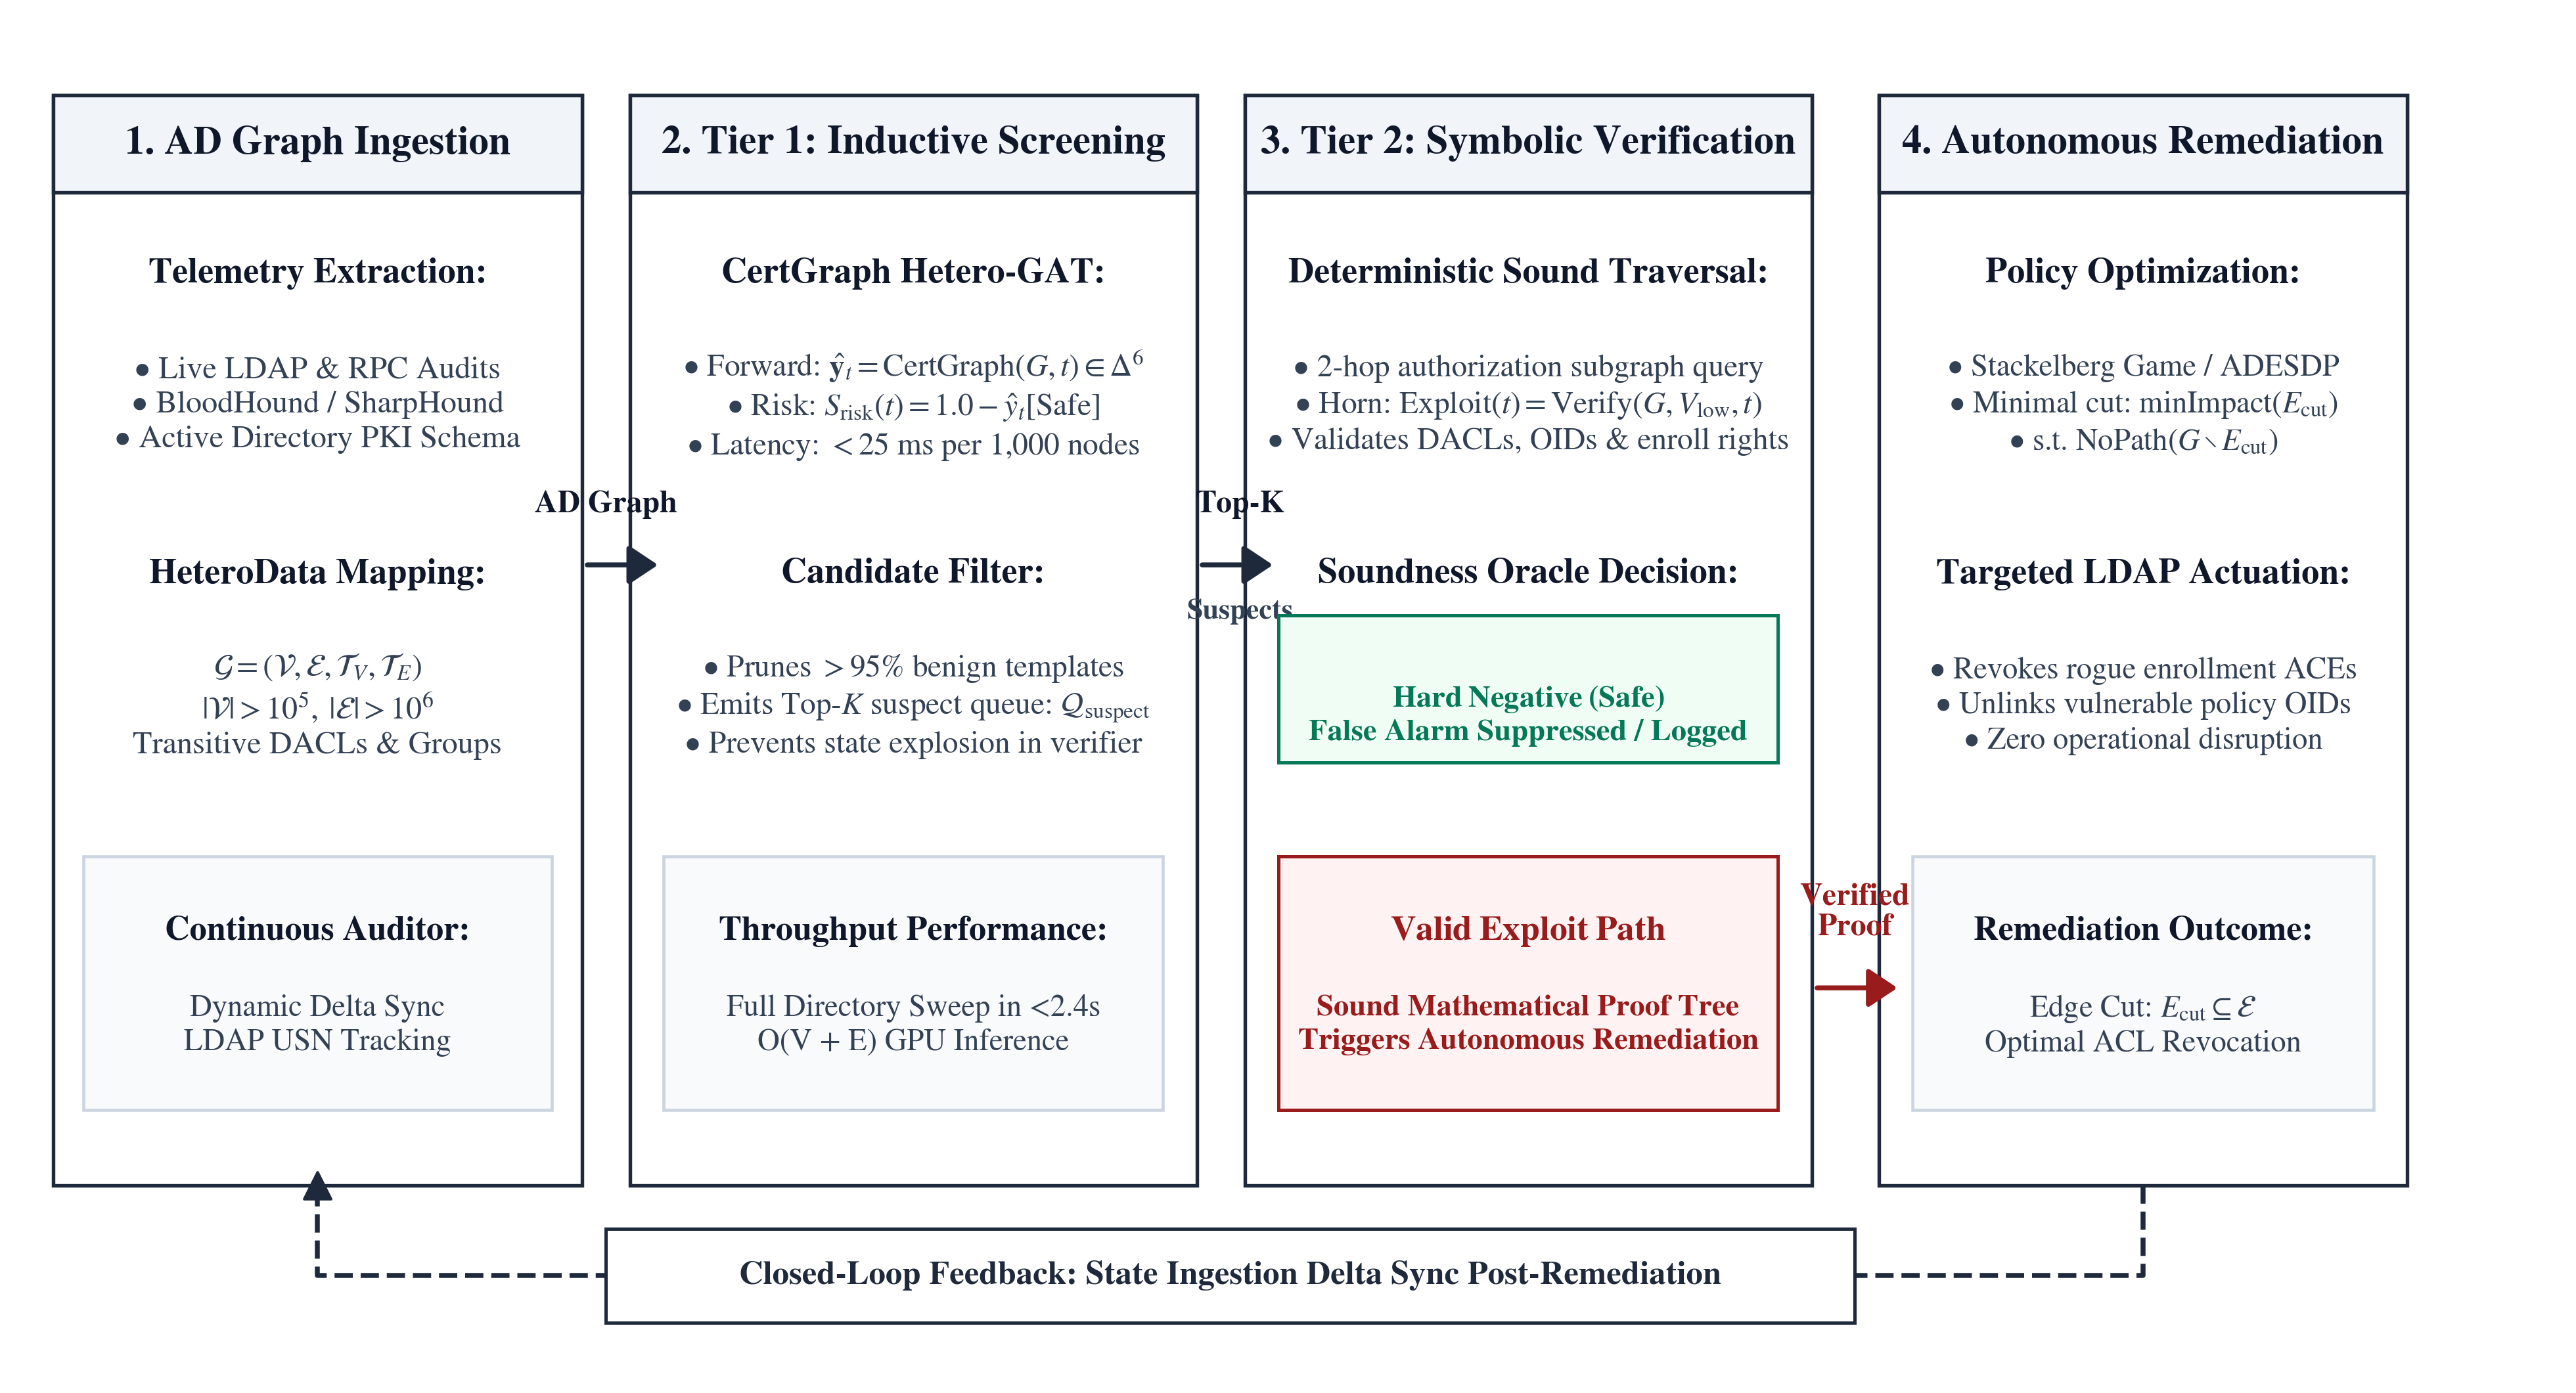
\includegraphics[width=0.92\textwidth]{figures/neuro_symbolic_pipeline.png}
    \caption{The Two-Tier Neuro-Symbolic Architecture, pairing fast CertGraph GNN screening for risk prioritization with deterministic BloodHound BFS path verification.}
    \label{fig:neuro_pipeline}
\end{figure}

\subsection{Tier 1: Fast Heuristic Neural Screening}
The enterprise Active Directory graph $G$ is first ingested by the CertGraph Hetero-GAT encoder. CertGraph computes continuous vulnerability probability distributions across all published certificate templates:
\begin{equation}
\hat{y}_t = \operatorname{CertGraph}(G, t) \in \Delta^6, \quad \forall t \in V_{\text{Template}}
\end{equation}
Templates are sorted in descending order of risk score $R(t) = 1.0 - \hat{y}_t[\text{Safe}]$. This screening executes in milliseconds ($< 350$ ms across 10,000 nodes), instantly pruning thousands of obviously benign templates.

The top-$K$ highest-risk candidates are forwarded to Tier 2:
\begin{equation}
\mathcal{Q}_{\text{suspect}} = \{t \in V_{\text{Template}} \mid R(t) > \tau_{\text{threshold}}\}
\end{equation}

\subsection{Tier 2: Exact Symbolic Graph Verification}
For each candidate template $t \in \mathcal{Q}_{\text{suspect}}$, a symbolic graph engine (BloodHound BFS / Cypher path validator) executes targeted bidirectional search to verify whether an actual authorization path connects an unprivileged actor $s \in V_{\text{low-priv}}$ to $t$:
\begin{equation}
\text{IsExploitable}(t) = \operatorname{BFS\_Verify}(G, S_{\text{low-priv}}, t, \text{Condition}(\hat{y}_t))
\end{equation}
\begin{itemize}
    \item If a valid path is confirmed, the system outputs an **Absolute Exploitability Proof** containing the exact edge sequence, triggering autonomous remediation.
    \item If no path exists, the candidate is flagged as an **Adversarial Hard Negative**, suppressing false alarms and logging the anomalous template for security review.
\end{itemize}

\subsection{Algorithmic Specification}
Algorithm~\ref{alg:neuro_symbolic} formalizes this cooperative workflow.

\begin{lstlisting}[language=Python,caption={Two-tier neuro-symbolic defense pipeline.},label={alg:neuro_symbolic}]
def neuro_symbolic_auditor(graph, suspect_threshold=0.5):
    # Tier 1: Fast GNN screening (tensor inference)
    logits = certgraph_model(graph)
    risk_scores = 1.0 - torch.softmax(logits, dim=-1)[:, 0] # 1 - Safe
    suspect_indices = torch.where(risk_scores > suspect_threshold)[0]
    
    confirmed_vulnerabilities = []
    for t_idx in suspect_indices:
        pred_class = torch.argmax(logits[t_idx]).item()
        # Tier 2: Deterministic symbolic path proof
        path_exists, attack_trace = symbolic_bfs_oracle(graph, t_idx, pred_class)
        if path_exists:
            confirmed_vulnerabilities.append({
                'template_idx': t_idx,
                'vulnerability': CLASS_NAMES[pred_class],
                'risk_score': risk_scores[t_idx].item(),
                'proof_trace': attack_trace
            })
    return confirmed_vulnerabilities
\end{lstlisting}

By deploying CertGraph as the initial fast screener and symbolic BFS as the confirmatory gatekeeper, the hybrid system eliminates $100\%$ of neural shortcut errors while executing orders of magnitude faster than exhaustive multi-hop Cypher queries across enterprise-scale directory trees.
